\documentclass[11pt, a4paper]{article}
%\usepackage{geometry}
\usepackage[inner=1.5cm,outer=1.5cm,top=2.5cm,bottom=2.5cm]{geometry}
\pagestyle{empty}
\usepackage{graphicx}
\usepackage{fancyhdr, lastpage, bbding, pmboxdraw}
\usepackage[usenames,dvipsnames]{color}
\definecolor{darkblue}{rgb}{0,0,.6}
\definecolor{darkred}{rgb}{.7,0,0}
\definecolor{darkgreen}{rgb}{0,.6,0}
\definecolor{red}{rgb}{.98,0,0}
\usepackage[colorlinks,pagebackref,pdfusetitle,urlcolor=darkblue,citecolor=darkblue,linkcolor=darkred,bookmarksnumbered,plainpages=false]{hyperref}
\renewcommand{\thefootnote}{\fnsymbol{footnote}}

\pagestyle{fancyplain}
\fancyhf{}
\lhead{ \fancyplain{}{CSC477: Introduction to Mobile Robotics - Assignment 3} }
%\chead{ \fancyplain{}{} }
%\rhead{ \fancyplain{}{Sept 25, 2019} }
%\rfoot{\fancyplain{}{page \thepage\ of \pageref{LastPage}}}
\fancyfoot[RO, LE] {page \thepage\ of \pageref{LastPage} }
\thispagestyle{plain}

%%%%%%%%%%%% LISTING %%%
\usepackage{listings}
\usepackage{caption}
\DeclareCaptionFont{white}{\color{white}}
\DeclareCaptionFormat{listing}{\colorbox{gray}{\parbox{\textwidth}{#1#2#3}}}
\captionsetup[lstlisting]{format=listing,labelfont=white,textfont=white}
\usepackage{verbatim} % used to display code
\usepackage{fancyvrb}
\usepackage{acronym}
\usepackage{amsthm}
\VerbatimFootnotes % Required, otherwise verbatim does not work in footnotes!



\definecolor{OliveGreen}{cmyk}{0.64,0,0.95,0.40}
\definecolor{CadetBlue}{cmyk}{0.62,0.57,0.23,0}
\definecolor{lightlightgray}{gray}{0.93}



\lstset{
  %language=bash,                          % Code langugage
  basicstyle=\ttfamily,                   % Code font, Examples: \footnotesize, \ttfamily
  keywordstyle=\color{OliveGreen},        % Keywords font ('*' = uppercase)
  commentstyle=\color{gray},              % Comments font
  numbers=left,                           % Line nums position
  numberstyle=\tiny,                      % Line-numbers fonts
  stepnumber=1,                           % Step between two line-numbers
  numbersep=5pt,                          % How far are line-numbers from code
  backgroundcolor=\color{lightlightgray}, % Choose background color
  frame=none,                             % A frame around the code
  tabsize=2,                              % Default tab size
  captionpos=t,                           % Caption-position = bottom
  breaklines=true,                        % Automatic line breaking?
  breakatwhitespace=false,                % Automatic breaks only at whitespace?
  showspaces=false,                       % Dont make spaces visible
  showtabs=false,                         % Dont make tabls visible
  columns=flexible,                       % Column format
  morekeywords={__global__, __device__},  % CUDA specific keywords
}

%%%%%%%%%%%%%%%%%%%%%%%%%%%%%%%%%%%%
\begin{document}
\begin{center}
  {\Large \textsc{CSC477 -- Introduction To Mobile Robotics \\ assignment 3, 15 points  \\ due: Nov 18, 2019, at 6pm}}
\end{center}
%\begin{center}
%Fall 2019, University of Toronto Mississauga
%\end{center}
%\date{September 26, 2014}

\setlength{\unitlength}{1in}
\renewcommand{\arraystretch}{2}

\noindent\textbf{Course Page:} \url{http://www.cs.toronto.edu/~florian/courses/csc477_fall19}

\vskip.15in
\noindent\textbf{Overview:} %\footnotemark
This assignment deals with estimation and mapping. You will implement occupancy grid mapping based on 2D LiDAR observations and known poses. You will also implement a simplified version of GraphSLAM for range observations to uniquely identifiable landmarks. Finally, you will write down the main components of an Extended Kalman Filter for a localization problem.

\section{Occupancy grid mapping (5pts)}
In this exercise you are going to implement parts of the occupancy grid mapping system discussed in class. In particular, you are going to map an environment
based on known odometry estimates and known 2D laser scans. Do \texttt{git pull} under your CSC477 repository to get the starter code. The functionality
that you need to implement is marked using to-do comments in the file \path{estimation_assignment/python/occupancy_grid_mapper.py}. To run your code,
\texttt{cd} \path{path/to/csc477_fall19/estimation_assignment} and execute the following commands on three different terminals:
\begin{verbatim}
rosbag play laser_and_odometry.bag
roslaunch  estimation_assignment occupancy_grid_mapping.launch                   
           odometry_orientation_noise_std_dev:=2.5 
           odometry_position_noise_std_dev:=0.1
rosrun rviz rviz    
\end{verbatim}
\quad
\newline
\noindent When rviz initializes, go to \path{File} $>$ \path{Open Config} and then load the configuration file in \path{estimation_assignment/resources/comp417.rviz}
which is going to start the visualization of laser scan messages, frames of reference, and debugging visualizations. Save this configuration file as the default
in your \path{/home/username/.rviz/default.rviz}, so you won't have to do this every time you restart rviz. In the \path{roslaunch} command given above, the standard deviation of the odometry orientation noise is given in degrees. In this example the true yaw of the robot is corrupted by random noise from $\mathcal{N}(0, 2.5^2)$. Similarly, the true position is corrupted by random noise from $\mathcal{N}(0, 0.1^2)$, which is expressed in meters. \path{laser_and_odometry.bag} is a recording of laser scans and odometry data in the environment you used in Assignment 1. The expected result for perfect odometry looks similar to Figure \ref{fig:gmapping}.
\newline
\begin{figure}[h!]
  \begin{center}
    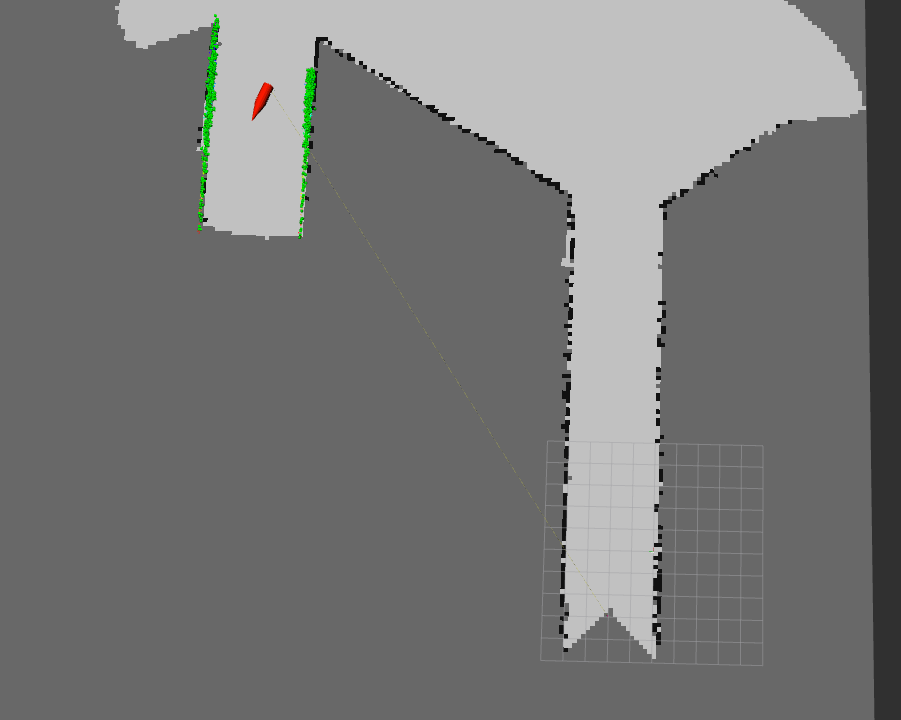
\includegraphics[width=0.3\textwidth]{gmapping}
  \end{center}
  \caption{Part of the robot's mapping task during the (0,0) noise trajectory.}
  \label{fig:gmapping}
\end{figure}
\newline
\newline
\noindent What you need to submit: 5 images of maps produced by your mapper, with noise parameters (0, 0), (2.5, 0), (5, 0), (2.5, 0.1), (5, 0.1) respectively.
Your images should be named \path{map_[0|1|2|3|4]_firstname_lastname.png}. Also, submit a video recording of the rviz visualization for the odometry noise combination (0,0),
demonstrating your map being built from beginning to end. Your video should be named \path{map_0_firstname_lastname.mp4/avi/ogg}.

\section{Least squares localization (5pts)}
In this exercise you are going to solve the localization problem in a map of known landmarks. In particular, assume your robot has 2D state $\textbf{x}_t=[p_x(t) \; p_y(t)]^T$ and an omnidirectional motion model $\textbf{x}_{t+1}=\textbf{x}_t + \textbf{u}_t\delta t + \textbf{w}_t$, where $\textbf{w}_t \sim \mathcal{N}(0, \sigma_w^2\textbf{I})$ is zero-mean Gaussian noise. The robot is moving through an environment that has L static landmarks $\textbf{l}_1, ..., \textbf{l}_L$ whose positions are known. Occasionally, the robot makes the following set of measurements: $z_t^{(i)}=||\textbf{x}_t-\textbf{l}_i||+n_t$ where $n_t \sim \mathcal{N}(0, \sigma_n^2)$, for some of the available landmarks.
Your goal is to estimate the sequence of states $\textbf{x}_{1:T}$ by minimizing a least squares cost function.
\newline
\newline
\noindent You can find starter code in \path{estimation_assignment/python/localization.py}. It provides the set of measurements made at each timesteps. Your task is to implement the cost
function using \path{numpy} and the nonlinear least squares solver in \path{scipy.optimize.least_squares}. There are to-do comments in the code that explain in detail what you need to implement.
After you are done with your implementation, the expected outcome is the following figure:
\begin{figure}[h]
  \begin{center}
    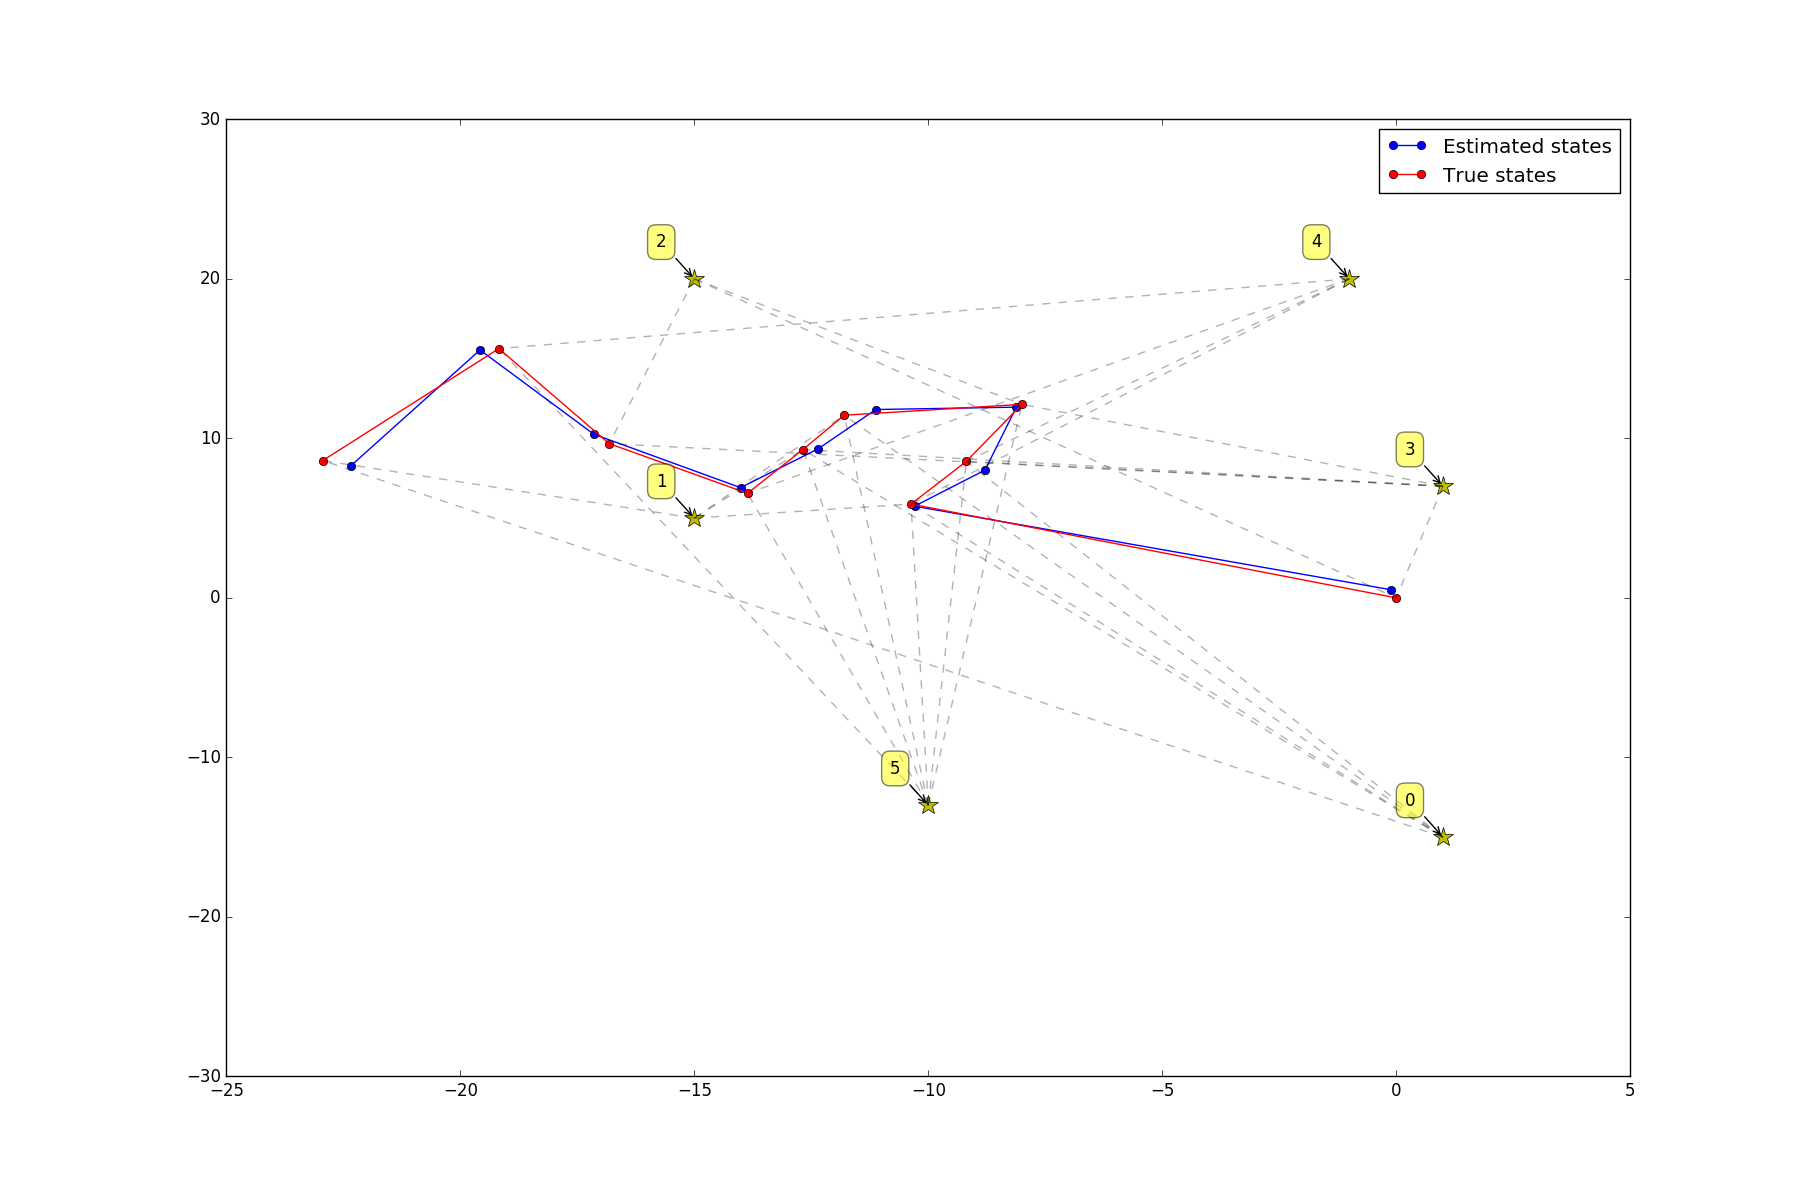
\includegraphics[width=\textwidth]{localization}
  \end{center}
  \caption{The robot starts at (0,0) and moves throughout the world, making measurements of static, known landmarks.}
\end{figure}

\noindent What you need to submit: your code in the file \path{estimation_assignment/python/localization.py}.
\newline
\newline
P.S.: You can think of cell phone localization based on static cell towers as a particular application of this problem.

\section{Extended Kalman Filter (5pts)}
Assume you have a robot that follows Dubins car dynamics on the plane. Its state is $\textbf{x}_t=[p_x(t) \; p_y(t) \; \theta(t)]$. Also assume that you have
three landmarks $\textbf{l}_i=[l_x^{(i)} \; l_y^{(i)}]$ in the world. At each point in time the robot observes all three landmarks, with some sensor noise.
The measurement model consists of the Euclidean distances from the robot's current state to each of the three landmarks, plus noise. Formulate an EKF estimator for this problem.
Specifically, formally define the dynamics model, the observation model, their Jacobians, and the covariances of their noise processes. There is no implementation
required for this question, but if you want to do it, you can find starter code at \path{path/to/csc477_fall19/filtering_examples/python}. Submit your work for this question as a pdf document or as a scanned image of your handwritten solution.

\section{How to submit}
Submit all your work in a file called \path{estimation_assignment.zip} that contains your extensions to the provided starter code, as well as the five images, the video, and the pdf file.
Submissions will be done on Quercus.

%%%%%% THE END
\end{document} 
